% Generated tables are read from notebook results by scripts/write_article.py.
\documentclass{psta}
\usepackage{graphicx}
\IfFileExists{paratype.sty}{\usepackage{paratype}}{}
\emergencystretch=2em
\tolerance=1600
\subjclass[UDC]{004.942}
\JournalRubric{8}
\def\russianPublicationInfo{Рабочая обезличенная рукопись. В редакцию не направлялась.}
\def\englishPublicationInfo{Anonymous working manuscript. Not submitted.}
\Russian
\title[Модель среды и прогноз задержек]{Исследование конфигурации краевой и туманной среды с прогнозированием задержек и выбором размещения связных задач}
\begin{abstract}
Представлена воспроизводимая дискретно-событийная модель трёхуровневой среды Edge--Fog--Cloud для исследования обработки событий мониторинга парковки. Модель учитывает отдельную очередь и конечный буфер каждого туманного узла, конкуренцию за каналы, потери и шесть составляющих сквозной задержки. Проведены серии изменения конфигурации и отдельные стрессовые испытания. При принятой суммарной интенсивности 400 событий в час ожидание в очереди в базовом прогоне отсутствует; ранее заявленные для другого исследования оптимальные размеры буфера и отношения числа датчиков к числу узлов не подтверждаются автоматически. Разработан единый интерфейс прогнозов с простыми методами, приближением очередей и демонстрационной нейросетью. Обучение, калибровка и проверка разделены по времени. На синтетической проверочной выборке нейросеть имеет меньшую среднюю абсолютную ошибку, но её верхний прогнозный порог не обеспечивает номинального покрытия 95\%. Показана связь прогноза с порядковыми командами и неизменённым алгоритмом выбора целых подграфов. Контрольные расчёты воспроизведены; в одном сквозном примере прогнозный вариант оказался медленнее базового. Результат представляет проверяемую среду исследования, а не доказательство универсального преимущества прогнозирования.
\end{abstract}
\keywords{краевые вычисления, туманные вычисления, дискретно-событийное моделирование, конечный буфер, прогноз задержки, связная задача, целые подграфы}
\English
\title[Environment model and delay forecasting]{Studying edge and fog environment configurations with delay forecasting and placement selection for connected tasks}
\begin{abstract}
A reproducible discrete-event model of an Edge--Fog--Cloud environment is presented for studying parking-monitoring events. The model represents an individual finite-buffer queue at each fog node, channel contention, losses, and six end-to-end delay components. Configuration sweeps and separate stress tests are performed. At the assumed total rate of 400 events per hour, the baseline run has no fog waiting time; buffer sizes and sensor-to-node ratios reported as optimal in a previous study therefore do not automatically carry over. A common forecast interface integrates simple predictors, a queueing approximation, and a demonstration neural network. Training, calibration, and evaluation are separated in time. On the synthetic test sample, the neural network has a lower mean absolute error, but its upper forecast threshold does not attain nominal 95\% coverage. Forecasts are connected to ordinal commands and an unchanged whole-subgraph placement algorithm. Control cases are reproduced; in one end-to-end interface example, the forecast-based choice is slower than the baseline. The contribution is a verifiable experimental environment, not proof of a universal advantage of forecasting.
\end{abstract}
\keywords{edge computing, fog computing, discrete-event simulation, finite buffer, delay forecasting, connected task, whole subgraphs}
\begin{document}
\Russian\maketitle
\hypertarget{english--authorsinfo}{}

\section{Введение}
Городские системы Интернета вещей объединяют распределённые датчики, локальную обработку и внешние сервисы хранения результатов. В мониторинге парковки требуется получить актуальное состояние места, не смешивая время доставки события с периодичностью обновления всей системы. Туманные вычисления рассматривают обработку между оконечными устройствами и облаком, а краевые вычисления приближают её к источнику данных~\cite{bonomi,shi}. Эти архитектурные идеи не задают конкретную задержку: она зависит от потока, обслуживания, каналов и правил размещения.

Исходным прикладным материалом служат предоставленные тезисы НСКФ-2026~\cite{nskf} «Исследование конфигурации вычислительной среды Edge-Fog». В них сообщаются средняя задержка 134,70 мс, 95-й перцентиль 170,90 мс, максимум 186,00 мс и среднее ожидание Fog 55,73 мс; туманный уровень назван узким местом, а увеличение числа облачных серверов в рассмотренных сериях не изменяет метрики. Это результаты \emph{предыдущей работы}, а не измерения предлагаемой программы. Полные выходные сведения тезисов требуют проверки до подачи статьи; DOI им не приписывается. Старый код не используется и не сверяется с новой реализацией.

Цель настоящей работы --- предоставить небольшую проверяемую модель для исследования конфигурации, сравнения прогнозов и демонстрации связи прогноза с выбором размещения связной задачи. Среда написана заново. Применимость формул очередей, происхождение параметров и границы выводов фиксируются явно. Из того, что в прежней серии масштабирование Cloud не давало эффекта, не следует универсальная бесполезность облака. Этот результат мотивирует принятую область \emph{изменяемого размещения} между Edge и Fog; Cloud остаётся фиксированным внешним уровнем результата. Такое разграничение сохраняется и в алгоритмическом примере.

Вклад состоит в воспроизводимой связке «среда --- наблюдения --- прогноз --- порядковые команды --- проверенный план». Он не включает новый обученный на реальном оборудовании прогнозировщик или доказательство ускорения относительно современных промышленных планировщиков. Работы~\cite{bonomi,shi} задают архитектурный контекст; они не являются источниками численных профилей эксперимента и не заменяют его валидацию. Положительные, нулевые и отрицательные эффекты конфигурации и прогноза сохраняются.

\subsection{Родственные работы и место исследования}
\paragraph{Среды моделирования.}
iFogSim~\cite{ifogsim} предназначен для исследования управления ресурсами IoT/Fog, включая задержки, сеть и стоимость. iFogSim2~\cite{ifogsim2} расширяет его средствами мобильности, кластеризации и микросервисов. EdgeCloudSim~\cite{edgecloudsim} ориентирован на экспериментальную оценку краевых вычислений, а YAFS~\cite{yafs} даёт программируемое описание распределённых IoT-сценариев и размещения. Эти инструменты шире нашей модели. Новое ядро не объявляется их заменой: его назначение --- прозрачная проверка отдельных очередей, допущений и связи с внешним прогнозным интерфейсом. Сравнения быстродействия этих симуляторов здесь не проводились.

\paragraph{Размещение и прогноз.}
HEFT~\cite{heft} связывает ранги задач с оценками вычислений и коммуникаций; наш краткий пример использует заданное разбиение и внешний порядок устройств, а не воспроизводит HEFT. Обзор размещения приложений в тумане~\cite{fogsurvey} показывает разнообразие ограничений и целей. Для FEFC этот обзор задаёт контекст явно ограниченной постановки части 3: фиксированное разбиение связной задачи и отдельная проверка ресурсных, сетевых и временных ограничений полного плана. Непрерывное декларативное рассуждение FogBrain~\cite{fogbrain} относится к пересмотру размещения при изменении среды. Wang и соавторы~\cite{wang} используют прогноз будущих затрат; отличие нашего интерфейса состоит в отделении численного прогноза отклика от порядковых команд и последующей обязательной проверки полного плана. Гарантии алгоритмов с прогнозным советом, например работы Wei~\cite{advice}, зависят от конкретной задачи и не переносятся на наш критерий автоматически. Работа Lykouris и Vassilvitskii~\cite{lykouris} о кэшировании с обученными подсказками служит основанием разделять полезность прогноза и поведение алгоритма при его ошибках; доказанные для кэширования гарантии конкурентности не переносятся на размещение FEFC.

\paragraph{Предсказание задержки и неопределённость.}
Для V2X исследовались сочетания машинного обучения и статистического прогноза задержки на данных поездок~\cite{v2x}; для потоковых вычислений --- архитектуры с механизмом внимания~\cite{chu}. Их объекты, данные и цели отличаются от синтетического MLP данной работы, поэтому опубликованные выигрыши не приписываются нашей модели. Выбор метрики требует учитывать шкалу и цель прогноза~\cite{hyndman}; здесь MAE оценивается на одной и той же выборке в миллисекундах. Квантильный порог оценивается отдельно от точечной ошибки. Split-conformal методы~\cite{lei,angelopoulos} задают конечновыборочную поправку при обменности наблюдений. Очередной временной ряд зависим и может смещаться, поэтому показывается фактическое покрытие, а не неподтверждённая гарантия 95\%.

\paragraph{Очереди и ограничения сопоставления.}
Модели очередей различаются законами поступлений, обслуживания и дисциплиной~\cite{kendall}. Равномерный сервис рассматриваемого имитатора не совпадает с экспоненциальным сервисом M/M/1/K. Закон Литтла~\cite{little} используется с интенсивностью принятых, а не всех поступивших задач. Аналитическая кривая служит проверяемым приближением, а не эталоном точного совпадения. Вклад настоящей работы --- воспроизводимое описание и проверка связи этих компонентов; мировой приоритет, превосходство над перечисленными системами и промышленная готовность не заявляются.


\section{Модель вычислительной среды}
\subsection{Уровни и обслуживание событий}
Модель содержит каждый из краевых датчиков, каждый туманный узел и каждый облачный сервер, а не один усреднённый Fog. Датчик с номером $i$ относится к зоне $i\bmod n_F$, где $n_F$ --- число Fog-узлов. Схема уровней приведена на рисунке~\ref{fig:architecture}. Отдельная очередь каждого Fog обслуживается в порядке поступления (FIFO). Буфер $B$ содержит только ожидающие задачи; вместе с одной обслуживаемой вместимость равна $K=B+1$. При заполнении ожидания новое событие теряется. Завершение обслуживания рассматривается перед поступлением при совпадении времён.

\begin{figure}\centering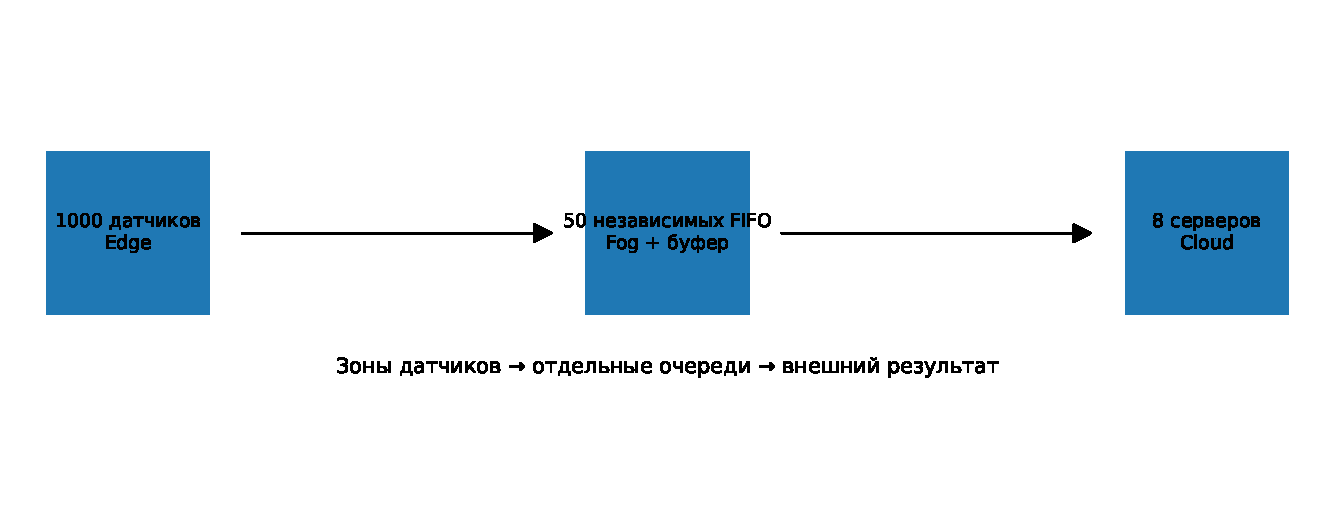
\includegraphics[width=\linewidth]{figures/architecture.pdf}
\caption{Группы устройств среды; в расчёте каждому Fog соответствует отдельная очередь. Тетрадь 01}\label{fig:architecture}\end{figure}

На каждом датчике последовательно выполняется обработка. У каждого Fog есть входной канал своей зоны и канал Fog--Cloud с отдельными календарями занятости. Облачный пул выбирает первый доступный сервер; при равенстве выбирается меньший номер. Передачи резервируются по готовности сообщения, облачная обработка --- по фактическому прибытию, а не по более раннему порядку генерации событий. Поэтому события из разных зон могут поступить в облако в изменённом порядке, не нарушая причинность.

Метки ESP32, Raspberry Pi 4, LoRaWAN/NB-IoT и HTTPS/MQTT взяты из прикладного сценария. Программа не эмулирует физический радиоканал, повторные передачи протокола, конкретные процессоры или криптографические затраты. Их влияние заменено заданными сервисными временами. Таблица~\ref{tab:parameters} отделяет параметры задания от новых допущений. Все интервалы в ней являются синтетическими профилями, не измерениями оборудования.

\begin{table}\caption{Базовые параметры и принятые допущения}\label{tab:parameters}\centering\small
\begin{tabular}{|p{32mm}|p{26mm}|p{44mm}|}\hline
Параметр & Значение & Основание\\ \hline
Число Edge/Fog/Cloud & 1000 / 50 / 8 & Прикладные тезисы, TASK\\ \hline
Edge: стационарный; мобильный & 5--15; 8--20 мс & Совместно обработка и передача; интерпретация TASK\\ \hline
Доля мобильных; доля обработки Edge & 0,30; 0,50 & Допущения модели\\ \hline
Fog; Cloud: обслуживание & 30--80; 10--30 мс & Диапазоны из задания\\ \hline
Fog--Cloud: сервис канала & 20--50 мс & Допущение\\ \hline
Закон сервисных времён & Равномерный & Допущение для каждого диапазона\\ \hline
Fog: мест ожидания & 400 & Базовое ограничение из задания\\ \hline
Суммарный поток; число событий & 400/ч; 200 & Задание; пуассоновский поток --- допущение\\ \hline
Начальное значение генераторов & 42 & Воспроизводимость контрольного прогона\\ \hline
\end{tabular}\end{table}

Интенсивность 400 событий в час относится ко \emph{всей системе}, а не к каждому датчику. Значение около 2000 транзакций в сутки описывает прикладной контекст и не приравнивается к круглосуточному пиковому потоку. Генерация заканчивается после заданного числа событий; затем все принятые события дообслуживаются. Временное окно поступлений и конец дренирования сохраняются отдельно. Это конечный эксперимент с пустым начальным состоянием, не оценка стационарного режима реальной парковки.

\subsection{Задержка и метрики}
Для завершённого события $j$ введём длительности обработки Edge $d^E_j$, передачи Edge--Fog $d^{EF}_j$, ожидания Fog $w^F_j$, обработки Fog $s^F_j$, передачи Fog--Cloud $d^{FC}_j$ и обработки Cloud $d^C_j$. Сквозная задержка определяется как
\begin{equation}\label{eq:latency}
y_j=d^E_j+d^{EF}_j+w^F_j+s^F_j+d^{FC}_j+d^C_j.
\end{equation}
В $d^E_j$ включено ожидание локального исполнителя, в $d^{EF}_j$ и $d^{FC}_j$ --- ожидание соответствующего канала, в $d^C_j$ --- ожидание облачного сервера. Эти ожидания также сохраняются отдельными полями. Таким образом, ровно шесть компонентов дают весь интервал от возникновения события до завершения, без скрытого добавления времени. Схема пути представлена на рисунке~\ref{fig:path}; равенство~\eqref{eq:latency} проверяется для каждого события.

\begin{figure}\centering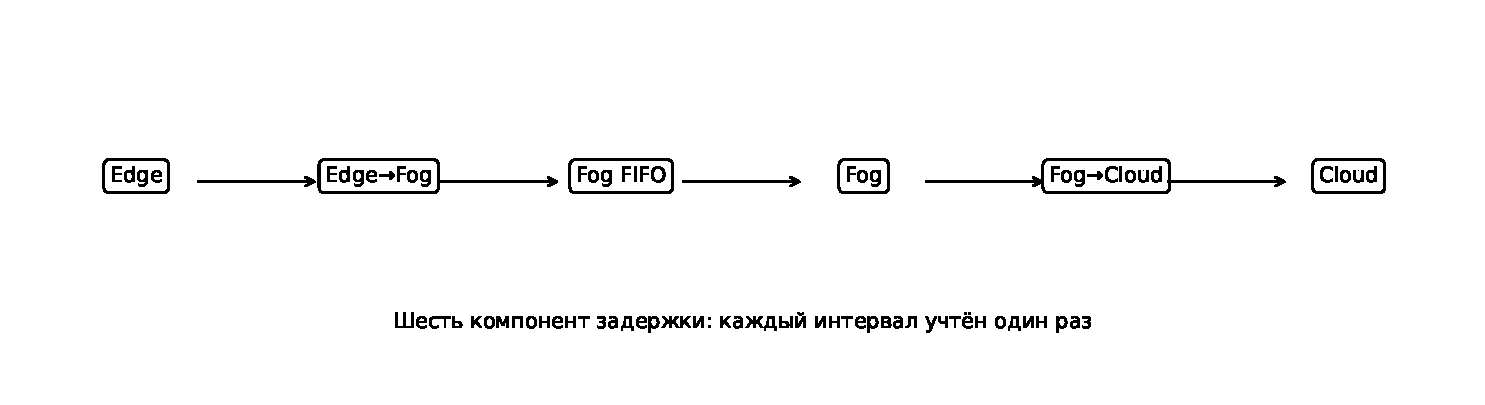
\includegraphics[width=\linewidth]{figures/six_path.pdf}
\caption{Путь события и шесть компонентов задержки. Тетрадь 01}\label{fig:path}\end{figure}

Пусть $m$ --- число завершённых событий, $y_{(1)}\le\ldots\le y_{(m)}$ --- упорядоченные задержки. Используется линейный эмпирический квантиль: при $h=1+(m-1)p$, $k=\lfloor h\rfloor$ и $k<m$
\begin{equation}\label{eq:quantile}
\widehat q_p=y_{(k)}+(h-k)(y_{(k+1)}-y_{(k)}),\qquad p=0{,}95.
\end{equation}
Для одного наблюдения квантиль равен ему, для пустой выборки не определён. Значение~\eqref{eq:quantile} характеризует выборку и не является гарантированным сроком. Среднее, максимум, вклады уровней и покрытие прогноза рассчитываются только для завершённых событий. Потери имеют отдельный счётчик и долю от всех поступивших; отсутствие задержки потерянного события не заменяется нулём.

Загрузка ресурса --- сумма его занятых интервалов, делённая на время от начала наблюдения до завершения дренирования. Это эмпирическая занятость модельного сервера или канала, а не измеренная загрузка физической сети. Порог 3 с применяется к задержке события; выполнение этого порога само по себе не доказывает обновление всех парковочных мест каждые 3 с.

\section{Методика экспериментов}
Тетрадь 01 формирует базовый запуск и однофакторные серии: увеличение Edge на 25--100\%, Cloud в два и три раза, Fog на 50\%, изменение буфера, доли мобильных датчиков и отношения датчиков к Fog в диапазоне 10--40. Всего задано 29 сценариев, включая отдельные стрессовые. При изменении числа Edge интенсивность пропорциональна его числу, то есть сохраняется средняя частота событий на датчик; число наблюдаемых событий остаётся 200. Изменяются и длительность наблюдения, и конечная реализация выборки типов. Поэтому малые колебания метрик не интерпретируются как доказанный эффект оптимизации.

Стрессовая серия использует суммарную интенсивность 1200 событий в секунду и 2000 поступлений при тех же 50 Fog. Она отделена от прикладного режима 400 событий в час. Буферы 0, 2, 20, 50, 100, 200 и 400 показывают работу переполнения и дренирования, а не рекомендуемый размер реального буфера.

Поступления, выбор зоны, датчика, его типа и профили времени имеют раздельные детерминированные генераторы. Изменение числа Cloud не меняет длительности задач, что позволяет парное сравнение этой серии. Одно начальное значение обеспечивает повторение заданного опыта, но не заменяет независимые повторения, доверительные интервалы или проверку чувствительности к распределениям. Число сценариев не выдаётся за число независимых статистических испытаний.

Прогнозная демонстрация в тетради 02 имеет собственный режим: 80 датчиков, четыре Fog, восемь Cloud, буфер 50 и 6000 событий при 60 событиях в секунду. Веса зон 4:2:1:1 создают неравномерную загрузку. Эти значения выбраны для проверки интерфейса в непустых очередях, а не для совпадения с численными ориентирами тезисов. Тетрадь 03 использует точный эталонный граф и один сквозной расчёт с выдачей сети, не выполняя развёрнутого сравнительного исследования алгоритма.

Схема «входы --- модель --- результаты» находится в тетради 01. Исходные CSV, параметры, временные отсечки, веса сети и планы сохраняются; отдельный реестр связывает каждый численный результат статьи с файлом и ячейкой. Чистые тетради и выполненные версии разделены. Все рисунки экспортируются только вызовами из тетрадей, а не рисуются по ожидаемым ответам. Эталонное ядро \texttt{v2/} контролируется по SHA-256 до и после запуска.

\section{Исследование конфигурации}
В базовом запуске завершены все 200 событий, потери отсутствуют. Средняя задержка равна @@BASEMEAN@@ мс, 95-й перцентиль --- @@BASEP95@@ мс, максимум --- @@BASEMAX@@ мс. Среднее ожидание Fog равно нулю. Результаты выбранных конфигураций приведены в таблице~\ref{tab:config}; первичные строки содержат все сценарии.

@@CONFIGTABLE@@

Нулевое ожидание не исправлялось искусственно. При равномерном распределении базового суммарного потока средняя интенсивность на Fog составляет $400/(3600\cdot50)$ события в секунду. Среднее обслуживание равно 0,055 с, поэтому номинальная предложенная нагрузка составляет около $1{,}22\cdot10^{-4}$ на узел. В конечной выборке очередь не образуется. В тезисах сообщалось 55,73 мс ожидания, но закон формирования такой очереди не задан полностью. Новая событийная модель не обязана воспроизводить это значение при иной явно определённой нагрузке.

Вклады уровней в новой базовой задержке: Edge --- @@EDGE_SHARE@@\%, Fog вместе с передачей в Cloud --- @@FOG_SHARE@@\%, Cloud --- @@CLOUD_SHARE@@\%. Компоненты показаны на рисунке~\ref{fig:components}. Большая доля Fog здесь связана с обслуживанием и передачей, а не с ожиданием в очереди. Термины «наибольший вклад» и «ресурс, ограничивающий пропускную способность» не отождествляются.
\begin{figure}\centering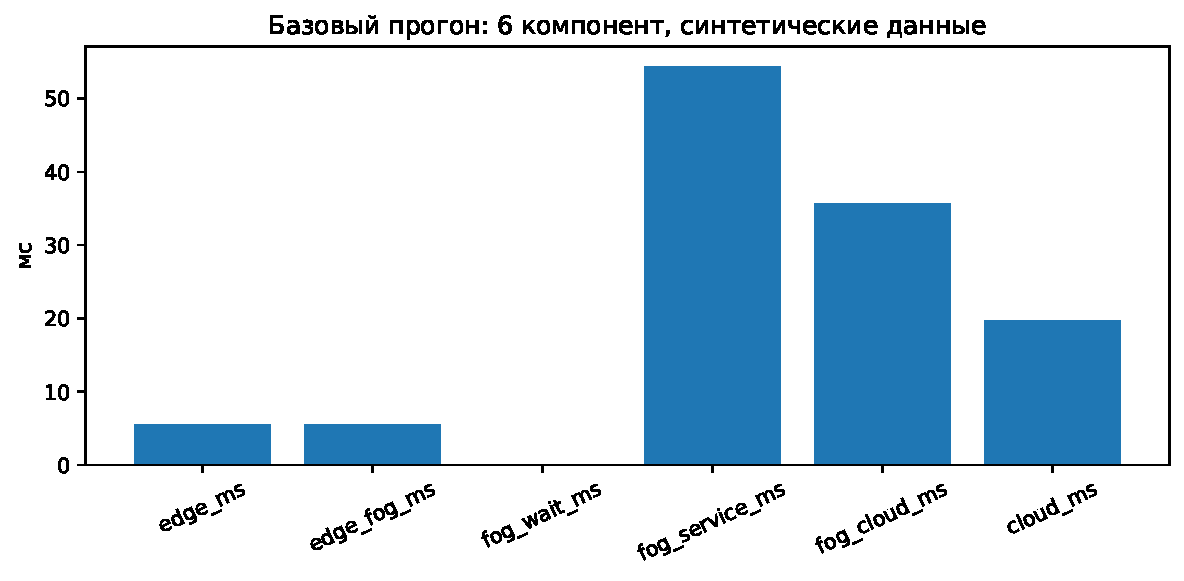
\includegraphics[width=.88\linewidth]{figures/components.pdf}
\caption{Разложение новой базовой задержки, не показатели предыдущей работы. Тетрадь 01}\label{fig:components}\end{figure}

В этой реализации базового потока увеличение Cloud до 16 и 24 не изменяет метрики: занятость слишком мала для появления ожидания Cloud. Это согласуется по направлению с прежним наблюдением, но не доказывает отсутствия облачного узкого места при другой нагрузке. Увеличение числа Fog до 75 также не даёт оснований заявлять ускорение по одному запуску без очереди. Стационарные и мобильные датчики различаются заданными диапазонами; результаты отражают эти предпосылки, а не измеренную мобильность оборудования.

В диапазоне 10--40 датчиков на Fog не обнаружен подтверждённый оптимум 20--25: средняя задержка меняется мало, а ожидание равно нулю. Буферы 20--400 в базовом режиме дают одинаковый результат. Поэтому прежняя рекомендация 50--100 не принимается за доказанный оптимум новой модели.

@@BUFFERTABLE@@

В стрессовой серии таблицы~\ref{tab:buffer} увеличение буфера уменьшает потери, но увеличивает задержки принятых задач. При малом буфере медленные события могут быть потеряны до получения целевой задержки; сравнение средних среди завершённых без доли потерь было бы смещённым. При буфере 50 и выше в данном конечном прогоне потерь нет, однако 95-й перцентиль превышает 3 с. Нельзя утверждать, что больший буфер одновременно улучшает все метрики. Очередь одного наиболее занятого узла на рисунке~\ref{fig:queue} является частью модели всех 50 узлов.
\begin{figure}\centering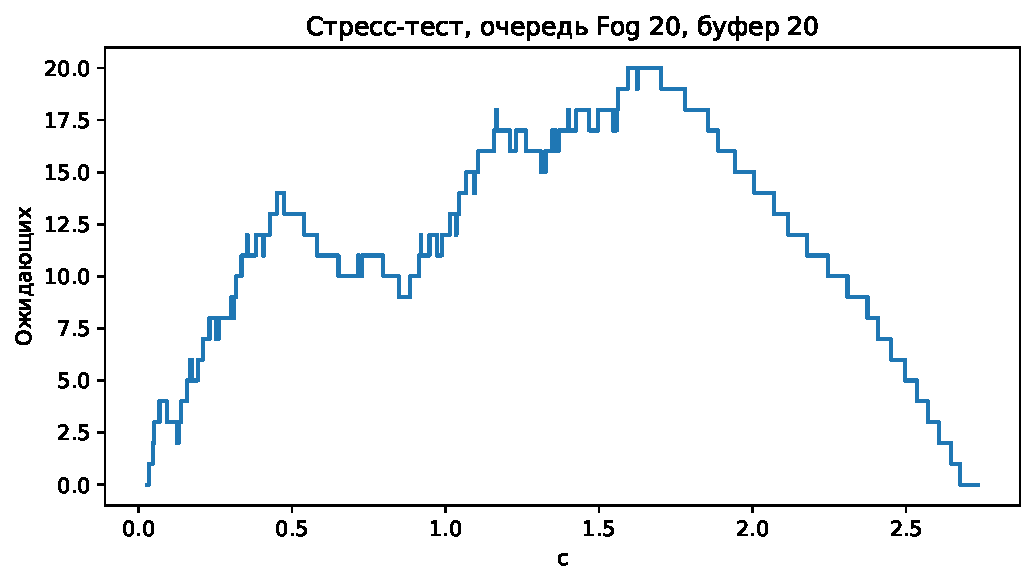
\includegraphics[width=.88\linewidth]{figures/queue.pdf}
\caption{Заполнение одного из отдельных Fog-буферов в стрессовом прогоне. Тетрадь 01}\label{fig:queue}\end{figure}

\section{Прогноз задержек и подключение нейросети}
\subsection{Единый интерфейс и причинность}
Все прогнозировщики предоставляют операции \texttt{fit(история)} и \texttt{predict(состояние)} с выходами \texttt{mean\_ms} и \texttt{p95\_ms}. Первый выход является точечным прогнозом задержки, а не известным истинным условным средним. Второй --- верхним прогнозным порогом с целевым покрытием 95\%. Замена модели не должна изменять смысл входов; пример адаптера для пользовательской сети включён в проект. Схема показана на рисунке~\ref{fig:socket}.
\begin{figure}\centering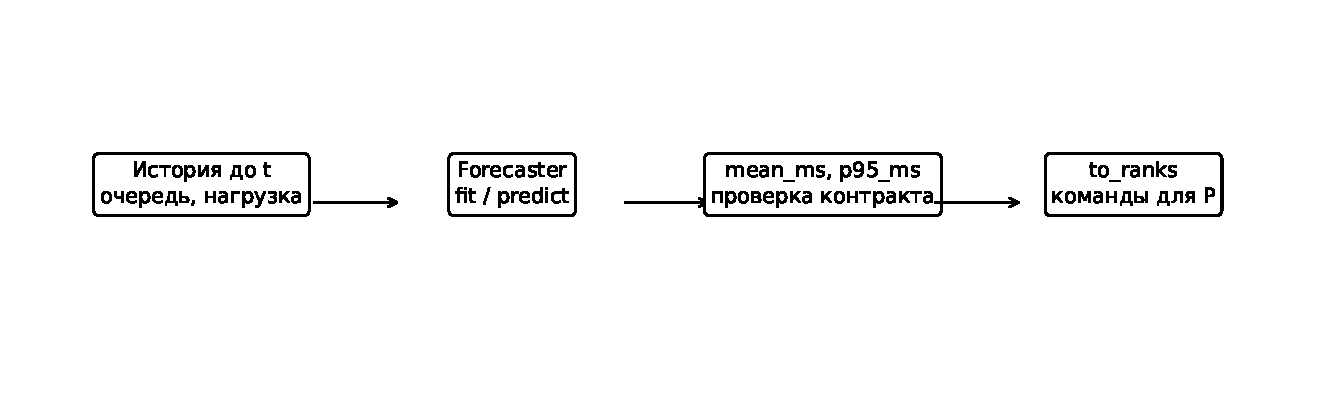
\includegraphics[width=\linewidth]{figures/forecast_socket.pdf}
\caption{Заменяемый прогнозный интерфейс и отдельное преобразование в ранги. Тетрадь 02}\label{fig:socket}\end{figure}

Признаки формируются при поступлении в Fog: число ожидающих, занятость исполнителя, оценка интенсивности, произведение этой оценки на среднее обслуживание, тип датчика и уже прошедшее время Edge с передачей. Истинная будущая задержка, будущие календари и известный симулятору остаток обслуживания в нейросеть не передаются.

Границы обучения и проверки определяются 60-м и 80-м процентилями времён поступления. В обучении используются только задачи, завершившиеся до первой границы; в калибровке --- поступившие после неё и завершившиеся до второй; проверка проводится на последующих поступлениях. Получены @@TRAINN@@ обучающих, @@CALN@@ калибровочных и @@TESTN@@ проверочных завершённых наблюдений. Из 6000 событий @@DROPPEDFORECAST@@ потеряны. Они не получают вымышленных задержек и не входят в покрытие; поэтому покрытие условно на завершённых задачах, а не является вероятностью успешной доставки любого события.

Naive использует последнее доступное наблюдение узла; MovingAverage --- среднее не более 32 последних; EWMA --- сглаживание с коэффициентом 0,2 по той же ограниченной истории. История обновляется только ответами, завершёнными до запроса. Эти правила одинаковы при калибровке и проверке; будущий ответ текущей задачи не входит в её признаки.

\subsection{Очередной прогноз и демонстрационный MLP}
Для приближённого метода Queueing принята модель M/M/1/K с интенсивностью $\lambda$, средней длительностью обслуживания $1/\mu$ и полной вместимостью $K$. Предложенная нагрузка $\rho=\lambda/\mu$ не равна фактической доле занятости при потерях. Стационарные вероятности числа задач $n$ имеют вид
\begin{equation}\label{eq:stationary}
 p_n=\begin{cases}\displaystyle\frac{(1-\rho)\rho^n}{1-\rho^{K+1}},&\rho\ne1,\\[4pt]
 \displaystyle\frac1{K+1},&\rho=1,\end{cases}\qquad 0\le n\le K.
\end{equation}
Формула~\eqref{eq:stationary} следует из баланса $\lambda p_n=\mu p_{n+1}$ и нормировки. Используемые численно логарифмические веса позволяют избежать переполнения при большой нагрузке. Пусть $L=\sum_{n=0}^{K}np_n$ --- среднее число задач, $\lambda_{\rm eff}$ --- интенсивность принятых задач, $W$ --- среднее время пребывания принятой задачи, $W_q$ --- её среднее ожидание. Для соответствующего стационарного приближения
\begin{equation}\label{eq:little}
\lambda_{\rm eff}=\lambda(1-p_K),\qquad
L=\lambda_{\rm eff}W,\qquad W_q=W-1/\mu.
\end{equation}
Закон Литтла~\cite{little} применяется к согласованным границам системы и потоку. В~\eqref{eq:little} потерянные задачи не входят в принятый поток; подстановка исходной $\lambda$ вместо $\lambda_{\rm eff}$ при блокировании была бы неверной. При нулевом потоке принимается предел $W=1/\mu$, $W_q=0$. Равномерный сервис и конечный стартовый прогон имитатора не совпадают с экспоненциальными стационарными предпосылками, поэтому Queueing --- приближённый сравнительный метод. К его оценке Fog добавляются уже известное Edge-время и принятые средние следующих стадий.

Демонстрационная нейросеть --- многослойный перцептрон с двумя скрытыми слоями 16 и 8 элементов. Масштабирование признаков и целевой величины оценивается только по обучению; начальное значение 42 и предел 350 итераций фиксированы. Ранняя остановка по случайно перемешанной проверочной выборке не используется. Сохранённые веса и параметры масштабирования позволяют повторить прямой проход без небезопасной загрузки исполняемого объекта. Это не новая промышленно обученная сеть и не доказательство преимущества выбранной архитектуры.

Для всех методов верхний порог строится одним способом. Если $\widehat y_j$ --- точечный прогноз, а $Q_{0.95}^{\rm cal}$ --- 95-й процентиль ошибок $y-\widehat y$ на калибровочном участке, то
\begin{equation}\label{eq:upper}
\widehat u_j=\widehat y_j+\max(0,Q_{0.95}^{\rm cal}).
\end{equation}
Здесь для калибровочных остатков выбирается наблюдаемая верхняя порядковая статистика, а не линейная интерполяция~\eqref{eq:quantile}; правило сохранено в коде. Из~\eqref{eq:upper} не следует гарантированное покрытие при изменении распределения или коррелированных наблюдениях. Для $m$ проверочных событий рассчитываются
\begin{equation}\label{eq:metrics}
\mathrm{MAE}=\frac1m\sum_{j=1}^{m}|y_j-\widehat y_j|,\qquad
\widehat C=\frac1m\sum_{j=1}^{m}\mathbf1\{y_j\le\widehat u_j\}.
\end{equation}
MAE в~\eqref{eq:metrics} сравнивает точечный прогноз с задержкой события, не с недоступным истинным условным ожиданием.

@@FORECASTTABLE@@

В таблице~\ref{tab:forecast} наименьшая MAE у демонстрационного MLP: @@MLPMAE@@ мс. Но покрытие @@MLPCOVER@@\% существенно ниже номинальных 95\%. Оно не исправлялось настройкой по проверочной выборке. Простое последнее наблюдение имеет большее покрытие при большей абсолютной ошибке. Эти метрики описывают разные свойства и не сводятся к единому утверждению о превосходстве сети. Большая ошибка Queueing указывает на ограниченность принятого приближения и оценки интенсивности в данном неравномерном конечном режиме, а не опровергает формулы очередей.
\begin{figure}\centering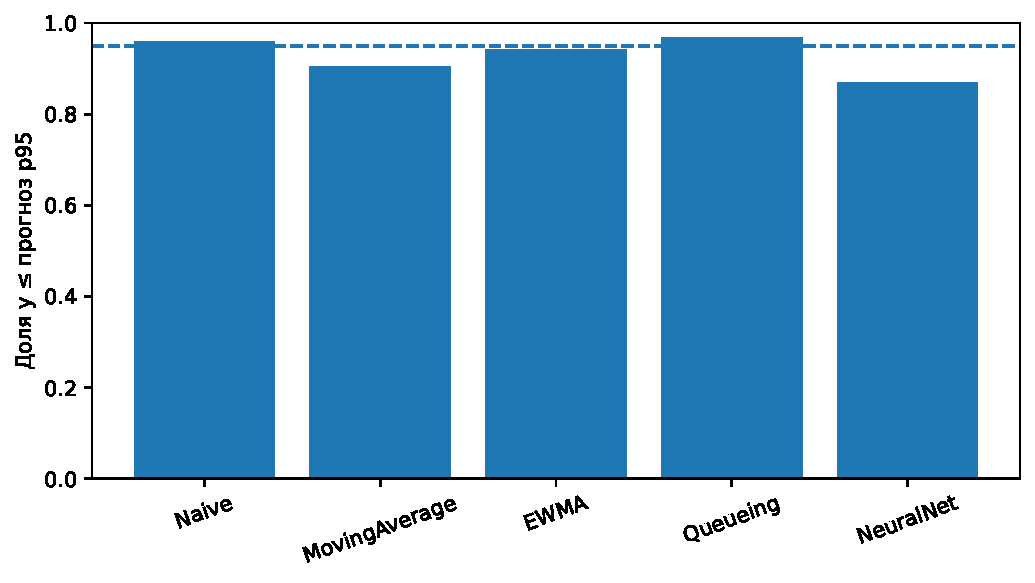
\includegraphics[width=.88\linewidth]{figures/forecast_coverage.pdf}
\caption{Эмпирическое покрытие верхнего порога; пунктир --- целевые 95\%. Тетрадь 02}\label{fig:coverage}\end{figure}

\section{Прогнозный алгоритм переразмещения}
\subsection{Неизменяемое ядро и правило выбора}
Пакет \texttt{v2/} используется непосредственно, без изменения поведения. Разбиение связной задачи фиксировано; размещаются целые подграфы, а не отдельные вершины внутри частей. Множество кандидатов ограничено Edge и Fog в принятой постановке. Обоснование исключения Cloud дано во введении; его нельзя подменять всеобщим утверждением, что облачная обработка не влияет на результат.

Для каждого устройства $d$ прогноз \texttt{mean\_ms} преобразуется в плотный порядковый ранг $c_d$: меньший прогноз получает меньшую команду, равные прогнозы --- равные команды. Эти команды определяют предпочтение и никогда не подставляются вместо физических длительностей блоков. Для назначения $\mu$ и $r$ целых подграфов формируется
\begin{equation}\label{eq:rank}
R(\mu)=\operatorname{sort}_{\downarrow}(c_{\mu(1)},\ldots,c_{\mu(r)}).
\end{equation}
Пусть $\mathcal P_{\rm ok}$ --- полные планы, прошедшие отдельную проверку ограничений; $T(P)$ --- расчётное время, $N(P)$ --- число переназначенных частей относительно прежнего назначения того же разбиения, $\operatorname{id}(P)$ --- устойчивый идентификатор. Выбор задаётся лексикографически:
\begin{equation}\label{eq:choice}
 P^*=\mathop{\operatorname{lexargmin}}_{P\in\mathcal P_{\rm ok}}
 (R(\mu_P),T(P),N(P),\operatorname{id}(P)).
\end{equation}
В базовом режиме B первый компонент отсутствует. D использует тот же критерий, что P, но порядок идентификаторов вместо прогнозного порядка. Неприменимый прогноз ведёт к B. При первичном размещении $N=0$ для всех планов; число переносов не является стоимостью миграции.

Для префикса назначения $z$ вычисляется оптимистический вектор $L(z)$, в котором неназначенным блокам сопоставлены минимальные разрешённые команды. Неотрицательность резервов памяти делает отсечение уже нарушенной памяти монотонным. Очередь упорядочена по $L$. Для найденного плана $\widehat P$ при непустой очереди остановка по прогнозному критерию разрешена только при
\begin{equation}\label{eq:stop}
\min_{z\in\mathrm{frontier}}L(z)>_{\rm lex}R(\mu_{\widehat P}).
\end{equation}
Равенство в~\eqref{eq:stop} не позволяет остановиться: время или последующие критерии могут улучшиться. При лимите поиска результат ограничен проверенными вариантами. Проверка полного плана учитывает совместимость, память, зависимости, маршруты, занятость ресурсов и срок. Она не вызывает построитель расписания, но имеет с ним общую модель; не является независимой физической валидацией инфраструктуры.

Рисунок~\ref{fig:placement} показывает границы интерфейсов. Переразмещение допускается до запуска или в явно заданной контрольной точке с сохранёнными данными. Живая миграция, переразбиение, скрытая передача состояния и непрерывный пересмотр во время исполнения не реализуются этим примером.
\begin{figure}\centering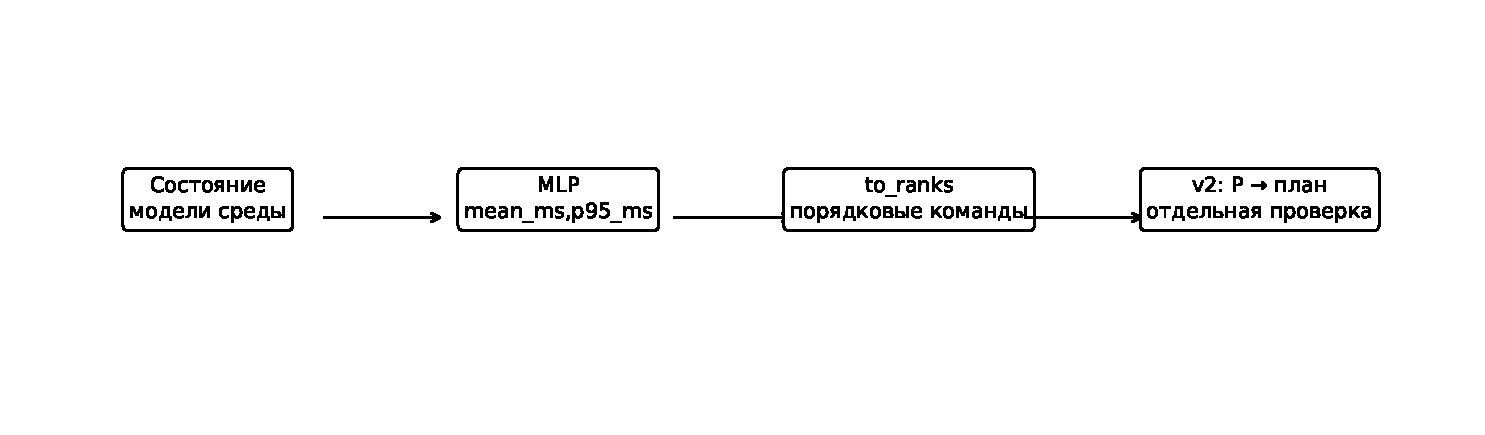
\includegraphics[width=\linewidth]{figures/placement_chain.pdf}
\caption{Связь модели среды, демонстрационной нейросети, порядковых команд и проверенного плана. Тетрадь 03}\label{fig:placement}\end{figure}

\subsection{Два коротких расчёта работоспособности}
В первом расчёте используется неизменённый синтетический пример эталона: цепь $a_1\to a_2\to b\to c$, части $A=\{a_1,a_2\}$, $B=\{b\}$, $C=\{c\}$. Время блоков на E равно 2, 5, 2 мс, на F --- 1, 2, 1 мс; память блоков --- 2, 3, 1 Мбайт, память устройств --- 4 и 6 Мбайт. Каждая удалённая передача занимает 1 мс. Команды E и F равны 1 и 2. Это тестовые значения, а не результат обученной сети.

@@CONTROLTABLE@@

Результаты таблицы~\ref{tab:controls} совпали точно. При сроке 3 мс невозможность в этом примере также следует из суммы минимальных последовательных длительностей $1+2+1=4$ мс ещё без передач. Вектору P приоритетно предпочтительно EFE, хотя FFF быстрее: критерий~\eqref{eq:choice} не равен минимизации одного времени. На рисунке~\ref{fig:graph} обе вершины A имеют одно назначение; интервалы на рисунке~\ref{fig:gantt} взяты из проверенного плана.
\begin{figure}\centering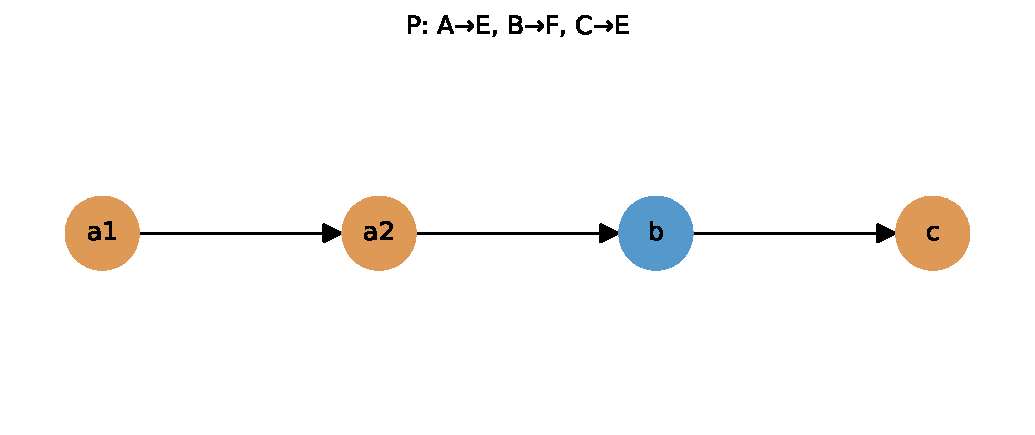
\includegraphics[width=.85\linewidth]{figures/graph_P.pdf}
\caption{Граф связной задачи с назначением целых частей для P; цвет обозначает устройство. Тетрадь 03}\label{fig:graph}\end{figure}
\begin{figure}\centering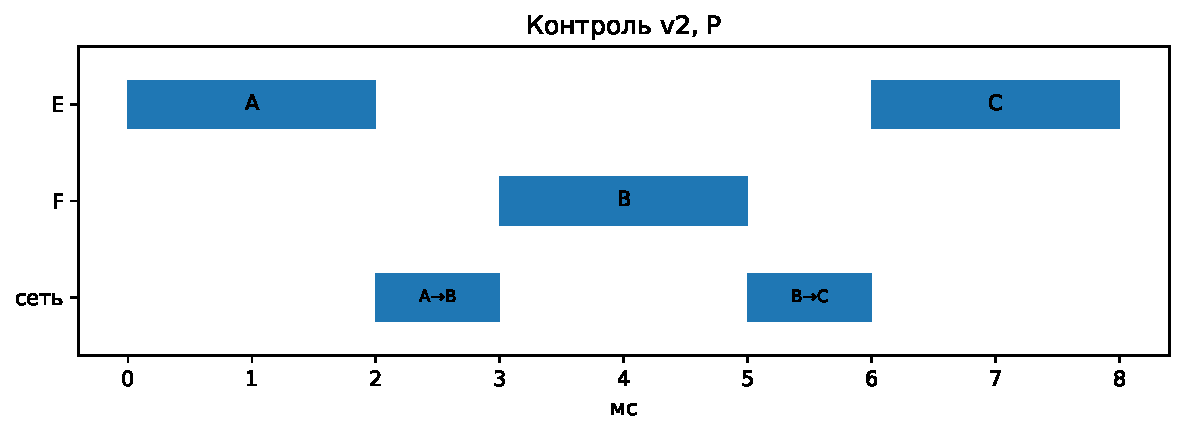
\includegraphics[width=.85\linewidth]{figures/gantt_P.pdf}
\caption{Вычисления и передачи контрольного плана P. Тетрадь 03}\label{fig:gantt}\end{figure}

Во втором расчёте загружаются сохранённые веса сети раздела 5. В момент начала проверочного участка выбираются заранее заданные Fog0 и Fog1 из зон с весами 4 и 2. Их очереди взяты из той же модели среды. Используются два Fog как подмножество допустимых E/F: сеть обучена на Fog-запросах, и перенос на иное Edge-оборудование без данных не предполагается.

Новый синтетический граф сохраняет разбиение, но время каждого блока принято равным 55 мс на обоих узлах; A состоит из двух операций по 27,5 мс. Доступно по 4 Мбайт памяти, суммарная потребность 6 Мбайт не допускает назначения всех блоков одному узлу. Сообщения 8000 бит, каналы 8 Мбит/с, срок 10 с --- явные допущения. Прогнозы полного отклика дают только ранги; профили блоков определены отдельно.

P и B получают один снимок оценочной фоновой занятости: $(q+0{,}5b)\cdot55$ мс, где $q$ --- число ожидающих, $b\in\{0,1\}$ --- занятость сервера; половина среднего сервиса для остатка --- допущение. Реализованный остаток ранее принятых задач передаётся только исполнителю. На протяжении короткого расчёта фон фиксирован, новые поступления не добавляются. Поэтому проверяется стык интерфейсов и календарное исполнение, а не полная онлайн-миграция в исходном потоке.

Сеть сформировала ранги @@RANKS@@. Результаты представлены в таблице~\ref{tab:linked}. Проверка исполнителя сохраняет назначение и маршруты, задерживая операции при занятости. В данном случае P медленнее B на @@DIFF@@ мс. Этот результат не удалён и не исправлен подбором состояния; один случай подтверждает выполнение связи «модель --- прогноз --- алгоритм», но не преимущество метода.

@@LINKEDTABLE@@

Проверены @@NEWTESTS@@ тестов нового пакета и 98 тестов неизменённого ядра; совпадение SHA-256 эталона проверяется до и после. Счётчики P/B в коротких примерах не используются как доказательство ускорения исполнения. Поведение и ограничения эталона, включая замечания рецензента, отдельно сопоставлены с утверждениями настоящей статьи.

\section{Заключение и ограничения}
Разработана новая дискретно-событийная среда с отдельными Fog-очередями, конечными буферами, календарями каналов и явным учётом потерь. Предоставлены выполненные тетради, проверяемые результаты и заменяемый прогнозный интерфейс. В базовом режиме малой суммарной интенсивности ожидание отсутствует; прежние рекомендации по буферу и отношению числа датчиков к Fog не подтверждаются автоматически. Стрессовые опыты показывают компромисс потерь и задержки, но не дают универсального оптимума.

Демонстрационный MLP на принятой синтетической выборке уменьшил MAE относительно выбранных простых методов, однако не обеспечил целевое покрытие p95. Связь с алгоритмом целых подграфов выполнена без подмены порядковых команд физическими характеристиками. Точные контрольные ответы воспроизведены, а единичный сквозной пример сохранил ухудшение P относительно B. Эти результаты ограничивают, а не расширяют без оснований область заявленных преимуществ.

Все параметры времени и новые события синтетические. Реальные протокольные эффекты, измеренные профили, независимая проверка обученной сети, стационарный анализ нагрузок, многократные статистические испытания и полноценная миграция остаются отдельными задачами. Недостающие выходные сведения конференционных тезисов, окончательный авторский состав и актуальность расширенного обзора должны быть подтверждены до подачи. Статья не объявляется готовой к публикации только по наличию запускаемого кода.

\raggedbottom
\paragraph{Доступность кода и данных.} Код, тетради, первичные CSV и журналы доступны в репозитории \url{https://github.com/annfridreksen/Forecast_Edge_Fog_Cloud}. Ветка --- \texttt{night/fefc-v3}. Исходный коммит выполненной сборки: \texttt{fc75e2a5119ed0b3d691961094fcc62998caf276}. Результаты публикуются отдельным последующим коммитом; его идентификатор и запуск приведены в PR~2 и \texttt{results/final-check.txt}. Эталон \texttt{v2/} не изменён.

\begin{thebibliography}{99}
\Bibitem{bonomi}
\by Bonomi Flavio, Milito Rodolfo, Zhu Jiang, Addepalli Sateesh
\paper Fog computing and its role in the internet of things
\jour Proceedings of the first edition of the MCC workshop on Mobile cloud computing
\yr 2012
\pages 13-16
\doi 10.1145/2342509.2342513

\Bibitem{shi}
\by Shi Weisong, Cao Jie, Zhang Quan, Li Youhuizi, Xu Lanyu
\paper Edge Computing: Vision and Challenges
\jour IEEE Internet of Things Journal
\vol 3
\issue 5
\yr 2016
\pages 637-646
\doi 10.1109/JIOT.2016.2579198

\RBibitem{nskf}
\by Игнатенко А. С., Орда-Жигулина М. В.
\paper Исследование конфигурации вычислительной среды Edge--Fog
\inbook Тезисы НСКФ-2026. Материал предоставлен авторами; выходные сведения уточняются. DOI не подтверждён
\yr 2026

\Bibitem{ifogsim}
\by Gupta Harshit, Vahid Dastjerdi Amir, Ghosh Soumya K., Buyya Rajkumar
\paper iFogSim: A toolkit for modeling and simulation of resource management techniques in the Internet of Things, Edge and Fog computing environments
\jour Software: Practice and Experience
\vol 47
\issue 9
\yr 2017
\pages 1275-1296
\doi 10.1002/spe.2509

\Bibitem{ifogsim2}
\by Mahmud Redowan, Pallewatta Samodha, Goudarzi Mohammad, Buyya Rajkumar
\paper iFogSim2: An extended iFogSim simulator for mobility, clustering, and microservice management in edge and fog computing environments
\jour Journal of Systems and Software
\vol 190
\yr 2022
\pages 111351
\doi 10.1016/j.jss.2022.111351

\Bibitem{edgecloudsim}
\by Sonmez Cagatay, Ozgovde Atay, Ersoy Cem
\paper EdgeCloudSim: An environment for performance evaluation of edge computing systems
\jour Transactions on Emerging Telecommunications Technologies
\vol 29
\issue 11
\yr 2018
\pages e3493
\doi 10.1002/ett.3493

\Bibitem{yafs}
\by Lera Isaac, Guerrero Carlos, Juiz Carlos
\paper YAFS: A Simulator for IoT Scenarios in Fog Computing
\jour IEEE Access
\vol 7
\yr 2019
\pages 91745-91758
\doi 10.1109/ACCESS.2019.2927895

\Bibitem{heft}
\by Topcuoglu H., Hariri S., Min-You Wu 
\paper Performance-effective and low-complexity task scheduling for heterogeneous computing
\jour IEEE Transactions on Parallel and Distributed Systems
\vol 13
\issue 3
\yr 2002
\pages 260-274
\doi 10.1109/71.993206

\Bibitem{fogsurvey}
\by Brogi Antonio, Forti Stefano, Guerrero Carlos, Lera Isaac
\paper How to place your apps in the fog: State of the art and open challenges
\jour Software: Practice and Experience
\vol 50
\issue 5
\yr 2020
\pages 719-740
\doi 10.1002/spe.2766

\Bibitem{fogbrain}
\by Forti Stefano, Bisicchia Giuseppe, Brogi Antonio
\paper Declarative continuous reasoning in the cloud-IoT continuum
\jour Journal of Logic and Computation
\vol 32
\issue 2
\yr 2022
\pages 206-232
\doi 10.1093/logcom/exab083

\Bibitem{wang}
\by Wang Shiqiang, Urgaonkar Rahul, He Ting, Chan Kevin, Zafer Murtaza, Leung Kin K.
\paper Dynamic Service Placement for Mobile Micro-Clouds with Predicted Future Costs
\jour IEEE Transactions on Parallel and Distributed Systems
\vol 28
\issue 4
\yr 2017
\pages 1002-1016
\doi 10.1109/TPDS.2016.2604814

\Bibitem{advice}
\by Wei Alexander
\paper Better and Simpler Learning-Augmented Online Caching
\jour LIPIcs, Volume 176, APPROX/RANDOM 2020
\vol 176
\yr 2020
\pages 60:1--60:17
\doi 10.4230/LIPIcs.APPROX/RANDOM.2020.60

\Bibitem{v2x}
\by Zhang Wenhan, Feng Mingjie, Krunz Marwan, Volos Haris
\paper Latency Prediction for Delay-sensitive V2X Applications in Mobile Cloud/Edge Computing Systems
\jour GLOBECOM 2020 - 2020 IEEE Global Communications Conference
\yr 2020
\pages 1-6
\doi 10.1109/GLOBECOM42002.2020.9348104

\Bibitem{chu}
\by Chu Zheng, Li Baozhu, Ying Changtian
\paper Transformer-based latency prediction for stream processing task
\jour Journal of King Saud University Computer and Information Sciences
\vol 37
\issue 5
\yr 2025
\pages 106
\doi 10.1007/s44443-025-00089-0

\Bibitem{hyndman}
\by Hyndman Rob J., Koehler Anne B.
\paper Another look at measures of forecast accuracy
\jour International Journal of Forecasting
\vol 22
\issue 4
\yr 2006
\pages 679-688
\doi 10.1016/j.ijforecast.2006.03.001

\Bibitem{lei}
\by Lei Jing, G’Sell Max, Rinaldo Alessandro, Tibshirani Ryan J., Wasserman Larry
\paper Distribution-Free Predictive Inference for Regression
\jour Journal of the American Statistical Association
\vol 113
\issue 523
\yr 2018
\pages 1094-1111
\doi 10.1080/01621459.2017.1307116

\Bibitem{angelopoulos}
\by Angelopoulos Anastasios N., Bates Stephen
\paper Conformal Prediction: A Gentle Introduction
\jour Foundations and Trends® in Machine Learning
\vol 16
\issue 4
\yr 2023
\pages 494-591
\doi 10.1561/2200000101

\Bibitem{kendall}
\by Kendall David G.
\paper Stochastic Processes Occurring in the Theory of Queues and their Analysis by the Method of the Imbedded Markov Chain
\jour The Annals of Mathematical Statistics
\vol 24
\issue 3
\yr 1953
\pages 338-354
\doi 10.1214/aoms/1177728975

\Bibitem{little}
\by Little John D. C.
\paper A Proof for the Queuing Formula:
                    L
                    = $\lambda$
                    W
\jour Operations Research
\vol 9
\issue 3
\yr 1961
\pages 383-387
\doi 10.1287/opre.9.3.383

\end{thebibliography}

\English\maketitle
\end{document}
